\section{System abstraction layer: dua-foundation}
\label{sec:dua_foundation}
The most important problem solved by DUA is also the first that it addresses: providing a similar environment across multiple system configurations. Achieving this is not a trivial task: the hardware platforms and operating systems that are of interest are very different from each other; yet, the aim is to provide an environment that offers the same OS APIs, libraries, and tools across all supported platforms. Nonetheless, DUA operates within the limits of what is possible without unnecessarily increasing any overheads: some aspects of the underlying hardware are not abstracted on purpose since it is not necessary to provide a consistent experience but instead implies introducing significant overheads in the execution of any application. This is the case of, \emph{e.g.}, the hardware architecture: as illustrated in the following, currently supported platforms include solutions based on both the x86-64 and ARM64 architectures, and the framework is designed to work on both of them without hiding them or their differences under an abstraction layer. This is due to multiple factors: first, there is no practical necessity to do so, and secondly, the developer using the framework can benefit of the peculiarities and specific features of each platform on which they want to deploy their software. Last but not least, abstracting the hardware architecture implies using hardware emulators such as QEMU \cite{bellard_qemu_nodate}, which are very powerful but also introduce significant overhead in the execution of any application, they are not always available on any platform, and they complicate access to system resources such as hardware devices which are instead of paramount importance in the practical contexts of this work, as shown in \Cref{tab:docker_features}.

This first part of DUA is called \texttt{dua-foundation} \cite{masocco_dua-foundation_nodate}, and is in essence a collection of Dockerfiles. The incipient intuition is that environments defined by a set of OS APIs and software tools can be easily replicated and managed in the form of Docker images, as described in \Cref{sec:docker}. Building a Docker image tailored to every supported platform allows the developer to account for the specific characteristics of each one, providing a consistent system configuration inside containers that use such images. Each researcher or developer, \emph{i.e.}, each \emph{user} of the DUA framework, has then to add their own software dependencies and packages to work on their specific modules. Let us call a user-developed software module based on DUA, a \emph{unit}. To define the system configuration that a unit requires, the Docker image is still the best tool available for the same reasons. For the sake of consistency along the whole chain, Docker images related to units have to start from the same set of base images as explained in \Cref{sec:docker}, which are the ones built from the Dockerfiles found in \texttt{dua-foundation}; the specific one is chosen depending on the hardware platform to work on. Let us then refer to images built from \texttt{dua-foundation} as to \emph{base units}.

The way a base unit is created differs even significantly for each, but the setup process they follow is the same for all. They all start from a platform-specific base image available on public registries like Docker Hub. Then, this image is enriched by a set of system packages which represent common dependencies in this field like, \emph{e.g.}, compilation toolchains. Finally, some more libraries are installed that are specific to the currently evaluated application areas of DUA: even if they may not be required by all units, they are included in the base units due to the frequency of their use in real-world scenarios, \emph{i.e.}, it is very likely to find different units that require them. At the end of the build process, each image is pushed on Docker Hub \cite{masocco_dotxautomationdua-foundation_nodate} to be available to all users of the framework.

To conclude, note that each supported hardware platform has its own base unit mainly to adapt the abstraction layer to the specific characteristics of the platform, but also to leverage and expose to the user the specific features of the platform itself. In fact, the aim of DUA base units is to provide \emph{similar} but not \emph{equivalent} environments: it is clarified in the following, when the currently supported platforms are presented, that some have specific resources that others lack. The framework is designed to work on all of them, but it is also designed to take advantage of the specific features of each one, and to expose those to the user in a consistent way. This is the reason why the setup process for each base unit is made of the same steps but performed differently each time, and why the resulting images are different from each other. It is then up to the user to develop their units on top of the base units that offer the best environment and features for their specific needs, depending on the specific requirements of the software contained in the unit.

The next sections explain the contents of \texttt{dua-foundation}: first, the set of software dependencies to be installed in every base unit is discussed, to describe what is the final system configuration achieved by every base unit. Then, currently supported hardware platforms are briefly illustrated, to show the variety of hardware that DUA integrates but also provide a first hint of the differences that the framework deals with. Finally, currently available base units are explained in more detail, together with the setup process that they follow.

\subsection{Common software dependencies}
\label{sec:dua_common_dependencies}
Providing here a full list of common software dependencies that are provided in every base unit is a daunting task. The interested reader can directly inspect the Dockerfiles in \cite{masocco_dua-foundation_nodate}. However, to give a general idea of the environment that base units provide, as well as to facilitate the inspection of their Dockerfiles, a summary of the most important software dependencies is provided here.

Each base unit starts from a set of system packages, that is, software packages that can be installed using the package manager of the Linux distribution that the base unit is built on, and provide basic functionalities. Since the distribution of choice for every base image is Ubuntu Linux, the package manager is \texttt{apt}; the choice of Ubuntu as first layer of every base unit is motivated by the same reasons given in \Cref{sec:dua_assumptions} and by the fact that an image containing a basic Ubuntu environment is relatively small in size, currently around \SI{30}{MB} \cite{canonical_ubuntu_nodate-1}. The first set of installed packages includes a GCC compilation toolchain \cite{free_software_foundation_gcc_nodate}, a Python system environment \cite{van_rossum_python_nodate}, a Java development kit \cite{oracle_java_nodate}, shell utilities, and a set of libraries that are required in the subsequent steps and that may depend on the specific base unit, as explained later on. These are installed now, all in a single command, to reduce the number of layers in the Docker image and improve its size, a well-established practice when building Docker images.

Next comes the middleware that is specific to the current main application areas of DUA, which are also subjects of this work and discussed in the next chapters. Usually, the first one to be installed among those is the \ROS middleware, presented in \Cref{sec:ros2}. The amount of \ROS packages installed depends on the target platform of a base unit: if the target is a development PC, a wide variety of packages is installed including simulators and visualizers, whereas if the target is a SBC, a reduced set of packages is installed skipping, \emph{e.g.}, visualization tools. Alongside a \ROS installation, DUA base units include both the eProsima Fast DDS \cite{eprosima_fast_nodate} and the Eclipse Cyclone DDS \cite{eclipse_foundation_cyclone_nodate} implementations of the DDS middleware presented in \Cref{sec:dds}, as well as the Zenoh middleware illustrated in \Cref{sec:zenoh}. This way, considering the intended application to distributed autonomous systems and the specific applications of robotics and real-time control architectures for nuclear fusion that are presented in this work, DUA base units offer to each user a complete set of tools to develop their software modules and build a distributed architecture.

Then is the time for the OpenCV computer vision library \cite{opencv_team_opencv_nodate,culjak_brief_2012} and the Eigen linear algebra library \cite{jacob_eigen_nodate}. The former is currently the de-facto standard in open-source computer vision, originally developed by Intel in the late 90s and then expanded by a vast team of developers, it now offers a wide range of functionalities and the implementation of thousands of algorithms ranging from image processing to mathematical operators. The latter is a C++ template library for linear algebra, which is widely used in the field of robotics and computer vision for its efficiency and ease of use. Finally, the Gazebo simulator presented in \Cref{sec:ros2_sim} is installed in base units for development systems.

The setup of a base unit concludes with specific tools that vary from time to time, depending on the evolution of application scenarios and supported platforms. Among these, the most important is currently the \texttt{dua-utils} collection, which is part of DUA and is illustrated in {\color{red}TODO dua-utils sec. ref.}. Their position at the end of the setup process is intended: these are the last stages of each Dockerfile contained in \cite{masocco_dua-foundation_nodate}, hence they correspond to the last layers in the image. This is done to allow to easily change these stages in case some tools are not needed or some new ones are to be added, without having to rebuild the whole image from scratch but only the last layers. This is another common practice in Docker image building, made possible by the ability of Docker to \emph{cache} image layers among subsequent builds, and it is used here to reduce the time required to build a base unit.

\subsection{Currently supported hardware platforms}
\label{sec:dua_supported_platforms}
To develop a framework that is applicable to a wide variety of practical cases, a good variety of hardware platforms has been considered for the initial implementation. The goal of this section is to present them in due detail, to show the variety of hardware that DUA integrates but also provide a first hint of the differences that the framework deals with. The categorization of the platforms made here is based on their system resources and intended use: it is not a strict classification, but a way to group them to better understand the differences among them. Note that, for simplicity, only 64-bit architectures are currently supported by DUA, as they have become the standard in the last decade and are now common in the microprocessor market. A real example is illustrated for almost all categories: such example items have also been used to test the framework and implement real autonomous systems prototypes during the development of this work. At the end of this section, \Cref{tab:dua_platforms} summarizes the most important system specifications of the example items, while some of the platforms that are supported by DUA, either fully or with some limitations as discussed above, are illustrated in \Cref{fig:duahw}.

\subsubsection{General-purpose PCs}
\label{sec:dua_supported_platforms_pc}
In the context of this work, this is the simplest category to address and also the most common. The first base units, as well as the other pieces of the DUA framework, have been put together and tested on this kind of platforms to ensure that the main concepts work. By \emph{general-purpose PC}, we mean a computer that is not specifically designed for a particular task, but that can be used for a wide variety of applications. This category includes desktop computers, laptops, and servers. In this context, it is assumed that among this category of systems, the ones that are of interest for this work are based on either the x86-64 or the ARM64 hardware architectures. In the practical and applicative contexts relevant to the DUA framework, these systems are used for development and testing purposes, as well as for running simulations and visualizations, or intensive real-time computations. The software tools that are used on these systems are the same as the ones that are used on the other platforms, but the hardware resources available on them are usually more powerful: many CPU cores, and much RAM and storage space are generally available. Dedicated coprocessors like, \emph{e.g.}, GPUs may also be available on these platforms.

\subsubsection{Single-board computers}
\label{sec:dua_supported_platforms_sbc}
In the field of autonomous systems, and especially in robotics, SBCs are very common. They are used in many applications, from small robots to drones, and they are also used in many research projects as fast prototyping platforms. The main reason for their popularity is that they are very cheap, small, and easy to use and integrate in larger systems, also thanks to their multiple communication interfaces. They are also very versatile, as they can be used for many different tasks. In the context of this work, SBCs are intended to be used to run the software modules that make an autonomous system perform its tasks. The hardware resources available here are generally more limited than the previous case, and GPUs and similar dedicated solutions may also not be available. This is also what makes SBCs so versatile in this field: their variety allows the system designer to choose the best solution that fits all the requirements, from software support, to mechanical constraints and energy consumption. In this work and for the explanatory purposes of this section, three classes of single-board computers are considered, making broad distinctions based on their hardware architecture and intended use.

The first class consists of single-board computers based on the ARM64 architecture. They are probably the most common and versatile type of SBC, due to some renowned features of the ARM architectures. First, ARM architectures usually have a very low power consumption, which makes them ideal for battery-powered applications. Second, their open design allows for a wide variety of implementations, which makes them very versatile and has paved the way for some very small but powerful implementations, perfect for SBCs and embedded systems. Last, ARM architectures have a very tidy instruction set, which contributes to both their low power consumption and high efficiency. The most famous ARM64 SBC is probably the Raspberry Pi series \cite{raspberry_pi_ltd_raspberry_nodate}, and DUA has been tested on the model 5.

The second class involves SBCs based on the x86-64 architecture. These are generally less common and more expensive than their ARM64 counterparts, since x86 processors are usually more powerful and have more features. They are usually employed for applications where more computational power is needed, or where the software that is going to be run on them is already available for x86 architectures. With respect to ARM-based SBCs, x86 ones usually have higher single-core frequencies and more cache memory, but at the price of higher power consumption. The selection of communication interfaces is also usually wider, and the support for peripherals is usually more complete, but each item on the board requires more power to operate. Moreover, the x86 architecture has been expanded over the years with many specific instruction sets, such as vector instruction sets like MMX, SSE, and AVX, which are very useful in many applications that require fast computations over large datasets. The most famous x86-64 SBC is probably the UP series \cite{aaeon_technology_up_nodate}, and DUA has been tested on the UP Squared and Xtreme models.

The last class is made by Nvidia Jetson SBCs \cite{nvidia_jetson_nodate}. These are ARM64-based solutions for edge computing on robotic systems, which also include a GPU, all integrated inside a Tegra SoC\footnote{System-on-Chip, a single chip that integrates all the components of a computer.}. The GPU is the most important feature of these SBCs, since it enables a wide variety of applications that require fast parallel computations ranging from image processing to object recognition and artificial intelligence models \cite{song_hardware_2024}. Many models and series have been released over the years, with models within a series being distinguished by their different set of system resources and price, so that customers can choose the solution that best suits their needs. The host system can be easily set up using the JetPack distribution by Nvidia \cite{nvidia_jetpack_nodate} which includes an OS installation based on Ubuntu, device drivers, and many Nvidia toolkits and SDKs\footnote{Software Development Kits.}. DUA has been tested on the Jetson Nano, TX2, Xavier NX, Xavier AGX, Orin NX, and Orin AGX models; as illustrated by this list, the employment of DUA on Jetson spanned over four series and six different models, showing the versatility of the framework. Different series, however, require different base units, due to both the host system configuration and the base image that is used to build the base unit: the setup process for each of them is described in the following. Note that, as shown in the following section, a specific JetPack version is used in every Jetson base unit image: to ensure compatibility with the hardware and software tools that are available on the Jetson platform, the JetPack version is chosen to be the one that is recommended by Nvidia for the specific model that the base unit is built for, and has to be the same that is actually installed on the host Jetson system.

\begin{table}[ht]
  \centering
  \makeatletter
  \begin{tabular}{|c|c|c|c|}
    \hline
    \textbf{SBC} & \textbf{CPU} & \textbf{RAM} & \textbf{GPU} \\
    \hline
    \textbf{Raspberry Pi 5} & \makecell{4c/4t Cortex-A76\\@ \SI{2.4}{\giga\hertz}} & \SI{8}{GB} & VideoCore VII \\
    \hline
    \textbf{Up$^2$} & \makecell{4c/4t Pentium N4200\\@ \SI{2.5}{\giga\hertz}} & \SI{8}{GB} & Intel HD Graphics \\
    \hline
    \textbf{Up Xtreme} & \makecell{4c/8t Core i7-8665UE\\@ \SI{4.4}{\giga\hertz}} & \SI{16}{GB} & Intel UHD Graphics \\
    \hline
    \textbf{Jetson Nano} & \makecell{4c/4t Cortex-A57\\@ \SI{1.43}{\giga\hertz}} & \SI{4}{GB} & \makecell{NVIDIA Maxwell\\128 CUDA cores} \\
    \hline
    \textbf{Jetson TX2} & \makecell{4c/4t Cortex-A57\\+\\2c/2t NVIDIA Denver 2\\@ \SI{1.95}{\giga\hertz}} & \SI{8}{GB} & \makecell{NVIDIA Pascal\\256 CUDA cores} \\
    \hline
    \textbf{\makecell{Jetson\\Xavier NX}} & \makecell{6c/6t NVIDIA Carmel\\ARM64 v8.2\\@ \SI{1.9}{\giga\hertz}} & \SI{16}{GB} & \makecell{NVIDIA Volta\\384 CUDA cores} \\
    \hline
    \textbf{\makecell{Jetson\\Xavier AGX}} & \makecell{8c/8t NVIDIA Carmel\\ARM64 v8.2\\@ \SI{2.2}{\giga\hertz}} & \SI{64}{GB} & \makecell{NVIDIA Volta\\512 CUDA cores} \\
    \hline
    \textbf{\makecell{Jetson\\Orin NX}} & \makecell{8c/8t Cortex-A78AE\\ARM64 v8.2\\@ \SI{2.0}{\giga\hertz}} & \SI{16}{GB} & \makecell{NVIDIA Ampere\\1024 CUDA cores} \\
    \hline
    \textbf{\makecell{Jetson\\Orin AGX}} & \makecell{12c/12t Cortex-A78AE\\ARM64 v8.2\\@ \SI{2.2}{\giga\hertz}} & \SI{64}{GB} & \makecell{NVIDIA Ampere\\2048 CUDA cores} \\
    \hline
  \end{tabular}
  \makeatother
  \caption{Summary of the technical specifications of some of the single-board computers currently supported by DUA.}
  \label{tab:dua_platforms}
\end{table}

\begin{figure}[t!]
  \centering
  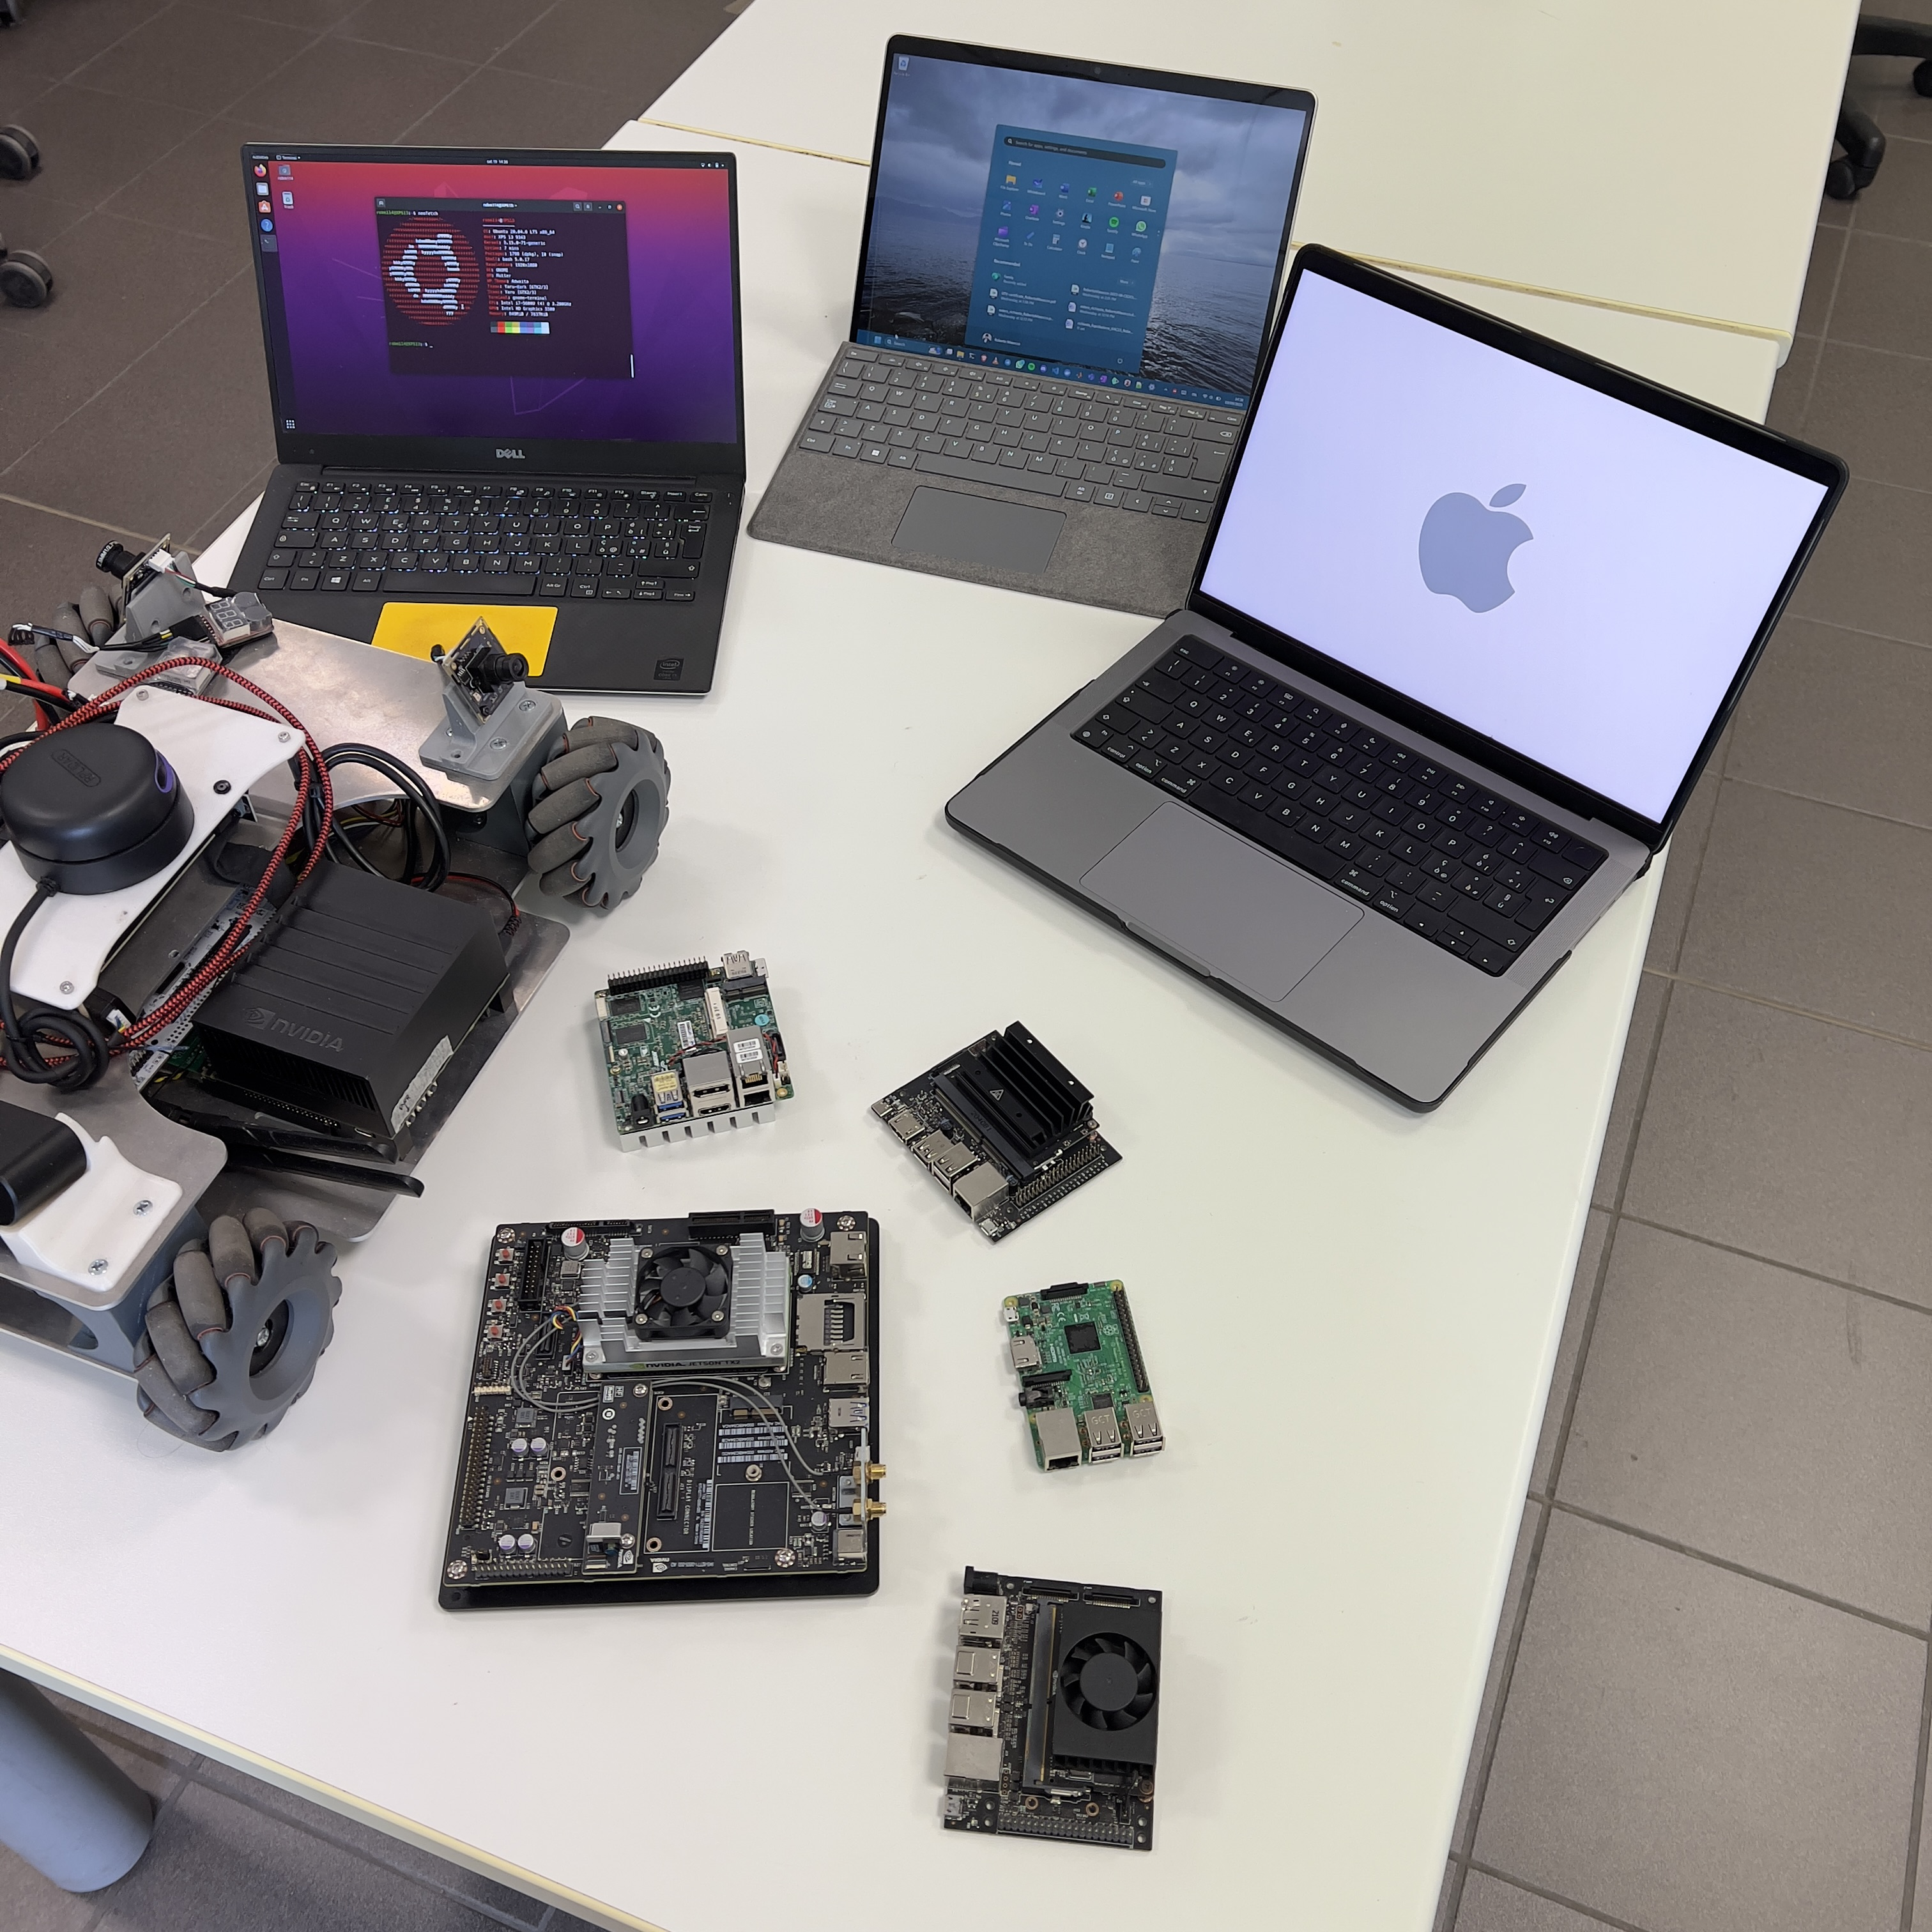
\includegraphics[width=0.8\textwidth]{images/ch4/duahw.png}
  \caption{Some of the platforms currently supported by DUA, either with full support or with some limitations as in \Cref{tab:docker_features}; from top left to bottom right: a Dell XPS 13 laptop, a Microsoft Surface tablet, a MacBook Pro, an Nvidia Jetson Xavier AGX mounted on a mobile robot prototype, an Up Squared, an Nvidia Jetson Nano, an Nvidia Jetson TX2 development kit, a Raspberry Pi, and an Nvidia Jetson Xavier NX.}
  \label{fig:duahw}
\end{figure}

\subsection{Base units}
\label{sec:dua_base_units}
\Cref{sec:dua_common_dependencies} and \Cref{sec:dua_supported_platforms} have presented the concept of base units, which are the building blocks of the DUA framework. They are Docker images that provide a consistent system configuration across all supported platforms, preserving the specific characteristics and features of the host platform wherever possible. Software modules, \emph{i.e.}, units built with DUA are then developed within containers whose images are built on top of these base units. \Cref{sec:dua_supported_platforms} has illustrated the currently supported hardware platforms, giving a general overview of their variety. It is now time to complete the description of the base units contained in \texttt{dua-foundation} by illustrating the setup process that each one follows in more detail, as well as the specific features that they offer to the user. Keep in mind that the description of each base unit can now be more detailed but not so long, since much of the setup process is common to all of them and has already been described in \Cref{sec:dua_common_dependencies}. Moreover, some base units are obtained by extending others, so the setup process for the former is a subset of the latter; this is the case of, \emph{e.g.}, base units for x86-64 systems and generic ARM64 systems, which can start with a configuration that suits a SBC, and then be evolved into a configuration that suits a development PC by adding more software tools, as anticipated in \Cref{sec:dua_common_dependencies}. One last thing to note is that, even if these particular base units could be built on top of each other by, \emph{e.g.}, obtaining the x86-64 development image starting from the x86-64 SBC image as described in \Cref{sec:docker}, this feature has not been employed and each base unit is built separately. This decision has been taken considering each build step that is performed in every such base unit, which led to this conclusion: installing some development tools for, \emph{e.g.}, \ROS or similar middleware after their core implementation has been installed in the SBC portion of the image forces Docker to go back to work on layers that have been already built, which slows down the build process and complicate the management of the image layers. Instead, building the base units separately allows to install the right set of packages in the right order and in single build steps, improving the image layers.

Before discussing each base unit in detail, a few words can be spent on the final sizes of the corresponding Docker images. \Cref{tab:dua_sizes} offers a summary of the sizes once the layers are compressed and stored on Docker Hub. As one can see, images can be quite large, reaching up to \SI{10}{GB} for the most complex development ones, with the ones for the SBCs being smaller and the ones for the Jetson systems being in the middle. The size of the images is not a concern for the framework, since they are not meant to be used directly by the user but only as a base for the development of software modules: as explained in \Cref{sec:docker}, even if multiple DUA images are built on a same host system, Docker reuses layers from the base unit since they are common to all images used on a host system. Regarding the build steps, the Dockerfiles in \cite{masocco_dua-foundation_nodate} show that care has been taken to reduce the size of the layers as much as possible by, \emph{e.g.}, installing packages using the minimum number of commands that is possible, and removing temporary files and build artifacts. The final size of the images is then a compromise between the need to provide a complete environment to the user and the need to keep the images as small as possible to reduce the time required to build them and the space required to store them. Development images are larger than the others because they include more tools, many of which have graphical elements, and Jetson ones are also the largest among those dedicated to SBCs since they include many specific libraries by Nvidia and third parties, as discussed below. Recall that the aim of this framework, in its current version and state, is to provide a complete, easy- and ready-to-use environment for research, development, and prototyping purposes: the size of the images as well of the amount of software tools that are installed in them are a consequence of this aim, in order to provide a complete, generic, and versatile environment.

\subsubsection{\texttt{x86-base}}
\label{sec:dua_base_units_x86-base}
The \texttt{x86-base} base unit is the simplest one, and it is intended to be used on SBCs based on the x86-64 architecture, as well as to deploy modules on general-purpose PCs when there is no need for additional development tools. It has also been the first one to be developed to test the framework. It starts from the official Ubuntu base image, and installs a set of system packages that are common to all base units, as described in \Cref{sec:dua_common_dependencies}. Since there is no need for additional development tools, the setup process ends here.

\subsubsection{\texttt{x86-dev}}
\label{sec:dua_base_units_x86-dev}
The \texttt{x86-dev} base unit is intended to be used on general-purpose PCs, and it is the one that is used to develop software modules that are intended to run on the x86-64 architecture. It starts from the same build stages of the \texttt{x86-base} base unit, adding in some of them development tools that are required to build software modules that are based on the \ROS middleware. Afterwards, the Gazebo simulator is also installed. Since this base unit is intended for a simple host platform, the setup process ends here.

\subsubsection{\texttt{x86-cudev}}
\label{sec:dua_base_units_x86-cudev}
This is where things start to get interesting, since this is the first image that accounts for peculiar characteristics of the host platform as well as for the specific features of the base image that is used to build the base unit. The \texttt{x86-cudev} base unit is intended to be used on general-purpose PCs based on the x86-64 architecture and that include an Nvidia GPU. They require a specific set of device drivers and libraries to be installed on the host system, as well as a specific Docker runtime to give them access to Nvidia GPUs on the host. The main difference is the base image: instead of a plain Ubuntu image, the \texttt{x86-cudev} base unit starts from the Nvidia CUDA+cuDNN base image, which is a Docker image based on Ubuntu that includes a CUDA Toolkit \cite{nvidia_cuda_nodate} and the cuDNN library and development files \cite{nvidia_cuda_nodate-1}. This is done to allow the user to develop software modules that can take advantage of the GPU on the host system, as well as many libraries that offer APIs ranging from parallel computations to machine learning. After the Nvidia ones, other libraries and tools aimed at machine learning and artificial intelligence are also installed, such as PyTorch \cite{pytorch_foundation_pytorch_nodate}, Keras \cite{chollet_keras_nodate}, ONNX \cite{linux_foundation_onnx_nodate}, TensorFlow \cite{google_brain_team_tensorflow_nodate}, and Ultralytics YOLO \cite{ultralytics_inc_ultralytics_nodate}. The installation of these and other Python libraries, here as well as in all the other base units, takes place inside a Python environment specifically created for DUA and that extends the system environment. The rest of the setup process is the same as the one for the \texttt{x86-dev} base unit, with the addition of some compilation options for libraries built from source such as, \emph{e.g.}, OpenCV, to enable GPU support.

\subsubsection{\texttt{armv8-base}}
\label{sec:dua_base_units_armv8-base}
The \texttt{armv8-base} base unit is the simplest one for ARM64-based SBCs, and it is intended to be used on them when there is no need for additional development tools. It starts from the official Ubuntu base image, and installs a set of system packages that are common to all base units as described in \Cref{sec:dua_common_dependencies}. The main difference of this base unit with respect to the \texttt{x86-base} one is that the build processes of libraries built from source such as, again, OpenCV are configured to take advantage of the ARM64 hardware architecture. This is another simple base unit so the setup process ends here.

\subsubsection{\texttt{armv8-dev}}
\label{sec:dua_base_units_armv8-dev}
The \texttt{armv8-dev} base unit, like its \texttt{x86-dev} counterpart, is intended to be used on general-purpose PCs running on ARM processors such as, \emph{e.g.}, Apple MacBook laptops with the recent Silicon series of SoCs. It starts from the same build stages of the \texttt{armv8-base} base unit, adding in some of them development tools that are required to build software modules that are based on the \ROS middleware. Afterwards, the Gazebo simulator is also installed. Source builds are again configured to take advantage of the ARM64 hardware architecture.

\subsubsection{\texttt{jetsonnano}}
\label{sec:dua_base_units_jetsonnano}
This is the first of the series of base units aimed at Jetson systems. Since they are all SBCs not particularly suited for on-board development, all the \texttt{jetson} base units starting from this one do not include development tools. The Jetson Nano is today an old platform, and its last compatible JetPack version is 4.6.2. At that time, Nvidia did not provide a base image for Docker, so the \texttt{jetsonnano} base unit starts from the official Ubuntu 20.04 base image and performs a series of steps that transform it into a JetPack installation corresponding to that version. The choice of Ubuntu 20.04 is motivated by the need to maintain compatibility with the Linux kernel version running on the Nano, which is 4.9 since JetPack 4.6.2 is based on Ubuntu 18.04. A JetPack installation is obtained by configuring some environment variables and configuration files, and adding Nvidia repositories to \texttt{apt} from which Nvidia packages are then downloaded. Then the setup process proceeds mostly as in the \texttt{armv8-base} base unit, with the addition of some Nvidia-specific packages and libraries that are required to run GPU-accelerated software on the Jetson and the source build of \ROS. In this image and the next \texttt{jetson} ones, building \ROS from source is required to keep its version consistent with the other base units: to use the most recent \ROS version available, in \texttt{x86} base units which are based on Ubuntu 22.04, the \ROS Debian packages are used to install the Humble Hawksbill version, while in \texttt{jetson} base units which are based on Ubuntu 20.04 the only way to install the same version is to build it from source. This is not a trivial task at all and requires many dependencies, build options and paths to be set correctly, but it is the only way to ensure that the same version of \ROS is used across all base units, which is a key requirement to ensure consistency of the environment provided by DUA.

\subsubsection{\texttt{jetsontx2}}
\label{sec:dua_base_units_jetsontx2}
The \texttt{jetsontx2} base unit is intended to be used on Jetson TX2 systems, and its setup process is almost identical to the one of the \texttt{jetsonnano} base unit. The main difference is that the JetPack version is 4.6.3, which is the last one compatible with the Jetson TX2.

\subsubsection{\texttt{jetson5}}
\label{sec:dua_base_units_jetson5}
This is the last of the series of base units aimed at Jetson systems, and thanks to recent support to Docker by Nvidia is one of the most simple to set up. It is meant to run on Jetson systems running a minor version of JetPack SDK version 5, a category which includes Xavier NX and AGX, and Orin NX and AGX. The base image is the official Nvidia JetPack SDK Docker image for machine learning, called \texttt{l4t-ml}, which is available from the Nvidia Container Registry \cite{nvidia_nvidia_nodate}. This image is based on Ubuntu 20.04, and includes a CUDA toolkit, cuDNN, and a set of libraries and tools for machine learning and artificial intelligence similar to that included in the \texttt{x86-cudev} base unit. Thus, the installation begins already as a JetPack environment, and what is left to install is the same set of tools and middleware as in the previous base units, set up in a similar way as in the other \texttt{jetson} base units.

\begin{table}[ht]
  \centering
  \makeatletter
  \begin{tabular}{|c|c|}
    \hline
    \textbf{Base unit} & \textbf{Docker image compressed size} \\
    \hline
    \texttt{armv8-base} & \SI{1.7}{GB} \\
    \hline
    \texttt{armv8-dev} & \SI{1.93}{GB} \\
    \hline
    \texttt{jetson5} & \SI{9.04}{GB} \\
    \hline
    \texttt{jetsonnano} & \SI{3.6}{GB} \\
    \hline
    \texttt{jetsontx2} & \SI{3.6}{GB} \\
    \hline
    \texttt{x86-base} & \SI{1.69}{GB} \\
    \hline
    \texttt{x86-cudev} & \SI{13.11}{GB} \\
    \hline
    \texttt{x86-dev} & \SI{2.96}{GB} \\
    \hline
  \end{tabular}
  \makeatother
  \caption{Sizes of the compressed Docker images of the base units currently available in \texttt{dua-foundation}.}
  \label{tab:dua_sizes}
\end{table}
